% Options for packages loaded elsewhere
\PassOptionsToPackage{unicode}{hyperref}
\PassOptionsToPackage{hyphens}{url}
%
\documentclass[
]{article}
\usepackage{amsmath,amssymb}
\usepackage{iftex}
\ifPDFTeX
  \usepackage[T1]{fontenc}
  \usepackage[utf8]{inputenc}
  \usepackage{textcomp} % provide euro and other symbols
\else % if luatex or xetex
  \usepackage{unicode-math} % this also loads fontspec
  \defaultfontfeatures{Scale=MatchLowercase}
  \defaultfontfeatures[\rmfamily]{Ligatures=TeX,Scale=1}
\fi
\usepackage{lmodern}
\ifPDFTeX\else
  % xetex/luatex font selection
\fi
% Use upquote if available, for straight quotes in verbatim environments
\IfFileExists{upquote.sty}{\usepackage{upquote}}{}
\IfFileExists{microtype.sty}{% use microtype if available
  \usepackage[]{microtype}
  \UseMicrotypeSet[protrusion]{basicmath} % disable protrusion for tt fonts
}{}
\makeatletter
\@ifundefined{KOMAClassName}{% if non-KOMA class
  \IfFileExists{parskip.sty}{%
    \usepackage{parskip}
  }{% else
    \setlength{\parindent}{0pt}
    \setlength{\parskip}{6pt plus 2pt minus 1pt}}
}{% if KOMA class
  \KOMAoptions{parskip=half}}
\makeatother
\usepackage{xcolor}
\usepackage[margin=1in]{geometry}
\usepackage{color}
\usepackage{fancyvrb}
\newcommand{\VerbBar}{|}
\newcommand{\VERB}{\Verb[commandchars=\\\{\}]}
\DefineVerbatimEnvironment{Highlighting}{Verbatim}{commandchars=\\\{\}}
% Add ',fontsize=\small' for more characters per line
\usepackage{framed}
\definecolor{shadecolor}{RGB}{248,248,248}
\newenvironment{Shaded}{\begin{snugshade}}{\end{snugshade}}
\newcommand{\AlertTok}[1]{\textcolor[rgb]{0.94,0.16,0.16}{#1}}
\newcommand{\AnnotationTok}[1]{\textcolor[rgb]{0.56,0.35,0.01}{\textbf{\textit{#1}}}}
\newcommand{\AttributeTok}[1]{\textcolor[rgb]{0.13,0.29,0.53}{#1}}
\newcommand{\BaseNTok}[1]{\textcolor[rgb]{0.00,0.00,0.81}{#1}}
\newcommand{\BuiltInTok}[1]{#1}
\newcommand{\CharTok}[1]{\textcolor[rgb]{0.31,0.60,0.02}{#1}}
\newcommand{\CommentTok}[1]{\textcolor[rgb]{0.56,0.35,0.01}{\textit{#1}}}
\newcommand{\CommentVarTok}[1]{\textcolor[rgb]{0.56,0.35,0.01}{\textbf{\textit{#1}}}}
\newcommand{\ConstantTok}[1]{\textcolor[rgb]{0.56,0.35,0.01}{#1}}
\newcommand{\ControlFlowTok}[1]{\textcolor[rgb]{0.13,0.29,0.53}{\textbf{#1}}}
\newcommand{\DataTypeTok}[1]{\textcolor[rgb]{0.13,0.29,0.53}{#1}}
\newcommand{\DecValTok}[1]{\textcolor[rgb]{0.00,0.00,0.81}{#1}}
\newcommand{\DocumentationTok}[1]{\textcolor[rgb]{0.56,0.35,0.01}{\textbf{\textit{#1}}}}
\newcommand{\ErrorTok}[1]{\textcolor[rgb]{0.64,0.00,0.00}{\textbf{#1}}}
\newcommand{\ExtensionTok}[1]{#1}
\newcommand{\FloatTok}[1]{\textcolor[rgb]{0.00,0.00,0.81}{#1}}
\newcommand{\FunctionTok}[1]{\textcolor[rgb]{0.13,0.29,0.53}{\textbf{#1}}}
\newcommand{\ImportTok}[1]{#1}
\newcommand{\InformationTok}[1]{\textcolor[rgb]{0.56,0.35,0.01}{\textbf{\textit{#1}}}}
\newcommand{\KeywordTok}[1]{\textcolor[rgb]{0.13,0.29,0.53}{\textbf{#1}}}
\newcommand{\NormalTok}[1]{#1}
\newcommand{\OperatorTok}[1]{\textcolor[rgb]{0.81,0.36,0.00}{\textbf{#1}}}
\newcommand{\OtherTok}[1]{\textcolor[rgb]{0.56,0.35,0.01}{#1}}
\newcommand{\PreprocessorTok}[1]{\textcolor[rgb]{0.56,0.35,0.01}{\textit{#1}}}
\newcommand{\RegionMarkerTok}[1]{#1}
\newcommand{\SpecialCharTok}[1]{\textcolor[rgb]{0.81,0.36,0.00}{\textbf{#1}}}
\newcommand{\SpecialStringTok}[1]{\textcolor[rgb]{0.31,0.60,0.02}{#1}}
\newcommand{\StringTok}[1]{\textcolor[rgb]{0.31,0.60,0.02}{#1}}
\newcommand{\VariableTok}[1]{\textcolor[rgb]{0.00,0.00,0.00}{#1}}
\newcommand{\VerbatimStringTok}[1]{\textcolor[rgb]{0.31,0.60,0.02}{#1}}
\newcommand{\WarningTok}[1]{\textcolor[rgb]{0.56,0.35,0.01}{\textbf{\textit{#1}}}}
\usepackage{longtable,booktabs,array}
\usepackage{calc} % for calculating minipage widths
% Correct order of tables after \paragraph or \subparagraph
\usepackage{etoolbox}
\makeatletter
\patchcmd\longtable{\par}{\if@noskipsec\mbox{}\fi\par}{}{}
\makeatother
% Allow footnotes in longtable head/foot
\IfFileExists{footnotehyper.sty}{\usepackage{footnotehyper}}{\usepackage{footnote}}
\makesavenoteenv{longtable}
\usepackage{graphicx}
\makeatletter
\def\maxwidth{\ifdim\Gin@nat@width>\linewidth\linewidth\else\Gin@nat@width\fi}
\def\maxheight{\ifdim\Gin@nat@height>\textheight\textheight\else\Gin@nat@height\fi}
\makeatother
% Scale images if necessary, so that they will not overflow the page
% margins by default, and it is still possible to overwrite the defaults
% using explicit options in \includegraphics[width, height, ...]{}
\setkeys{Gin}{width=\maxwidth,height=\maxheight,keepaspectratio}
% Set default figure placement to htbp
\makeatletter
\def\fps@figure{htbp}
\makeatother
\setlength{\emergencystretch}{3em} % prevent overfull lines
\providecommand{\tightlist}{%
  \setlength{\itemsep}{0pt}\setlength{\parskip}{0pt}}
\setcounter{secnumdepth}{-\maxdimen} % remove section numbering
\ifLuaTeX
  \usepackage{selnolig}  % disable illegal ligatures
\fi
\IfFileExists{bookmark.sty}{\usepackage{bookmark}}{\usepackage{hyperref}}
\IfFileExists{xurl.sty}{\usepackage{xurl}}{} % add URL line breaks if available
\urlstyle{same}
\hypersetup{
  pdftitle={CSC 587 HW 4},
  pdfauthor={Daniel R. Getty},
  hidelinks,
  pdfcreator={LaTeX via pandoc}}

\title{CSC 587 HW 4}
\author{Daniel R. Getty}
\date{2024-04-22}

\begin{document}
\maketitle

\hypertarget{homework-4}{%
\subsection{Homework 4}\label{homework-4}}

\begin{enumerate}
\def\labelenumi{\arabic{enumi}.}
\tightlist
\item
  Given a data tuple having the values ''systems'', ''26\_30'', and
  ''46K\_50K'' for the attributes department, age, and salary,
  respectively, what would a naive Bayesian classification of the status
  according to the data above? Notice that Count column is NOT an
  attribute. It just tells how many times a row occurs in our database
  and status is our target variable.
\end{enumerate}

\begin{Shaded}
\begin{Highlighting}[]
\CommentTok{\# create a data frame}
\NormalTok{data }\OperatorTok{=}\NormalTok{ \{}\StringTok{\textquotesingle{}department\textquotesingle{}}\NormalTok{: [}\StringTok{\textquotesingle{}sales\textquotesingle{}}\NormalTok{, }\StringTok{\textquotesingle{}sales\textquotesingle{}}\NormalTok{, }\StringTok{\textquotesingle{}sales\textquotesingle{}}\NormalTok{, }\StringTok{\textquotesingle{}systems\textquotesingle{}}\NormalTok{, }\StringTok{\textquotesingle{}systems\textquotesingle{}}\NormalTok{, }\StringTok{\textquotesingle{}systems\textquotesingle{}}\NormalTok{, }\StringTok{\textquotesingle{}systems\textquotesingle{}}\NormalTok{, }\StringTok{\textquotesingle{}marketing\textquotesingle{}}\NormalTok{, }\StringTok{\textquotesingle{}marketing\textquotesingle{}}\NormalTok{, }\StringTok{\textquotesingle{}secretary\textquotesingle{}}\NormalTok{, }\StringTok{\textquotesingle{}secretary\textquotesingle{}}\NormalTok{],}\StringTok{\textquotesingle{}age\textquotesingle{}}\NormalTok{: [}\StringTok{\textquotesingle{}31\_35\textquotesingle{}}\NormalTok{, }\StringTok{\textquotesingle{}26\_30\textquotesingle{}}\NormalTok{, }\StringTok{\textquotesingle{}31\_35\textquotesingle{}}\NormalTok{, }\StringTok{\textquotesingle{}21\_25\textquotesingle{}}\NormalTok{, }\StringTok{\textquotesingle{}31\_35\textquotesingle{}}\NormalTok{, }\StringTok{\textquotesingle{}26\_30\textquotesingle{}}\NormalTok{, }\StringTok{\textquotesingle{}41\_45\textquotesingle{}}\NormalTok{, }\StringTok{\textquotesingle{}36\_40\textquotesingle{}}\NormalTok{, }\StringTok{\textquotesingle{}31\_35\textquotesingle{}}\NormalTok{, }\StringTok{\textquotesingle{}46\_50\textquotesingle{}}\NormalTok{, }\StringTok{\textquotesingle{}26\_30\textquotesingle{}}\NormalTok{],}\StringTok{\textquotesingle{}salary\textquotesingle{}}\NormalTok{: [}\StringTok{\textquotesingle{}46K\_50K\textquotesingle{}}\NormalTok{, }\StringTok{\textquotesingle{}26K\_30K\textquotesingle{}}\NormalTok{, }\StringTok{\textquotesingle{}31K\_35K\textquotesingle{}}\NormalTok{, }\StringTok{\textquotesingle{}46K\_50K\textquotesingle{}}\NormalTok{, }\StringTok{\textquotesingle{}66K\_70K\textquotesingle{}}\NormalTok{, }\StringTok{\textquotesingle{}46K\_50K\textquotesingle{}}\NormalTok{, }\StringTok{\textquotesingle{}66K\_70K\textquotesingle{}}\NormalTok{, }\StringTok{\textquotesingle{}46K\_50K\textquotesingle{}}\NormalTok{, }\StringTok{\textquotesingle{}41K\_45K\textquotesingle{}}\NormalTok{, }\StringTok{\textquotesingle{}36K\_40K\textquotesingle{}}\NormalTok{, }\StringTok{\textquotesingle{}26K\_30K\textquotesingle{}}\NormalTok{], }\StringTok{\textquotesingle{}status\textquotesingle{}}\NormalTok{: [}\StringTok{\textquotesingle{}senior\textquotesingle{}}\NormalTok{, }\StringTok{\textquotesingle{}junior\textquotesingle{}}\NormalTok{, }\StringTok{\textquotesingle{}junior\textquotesingle{}}\NormalTok{, }\StringTok{\textquotesingle{}junior\textquotesingle{}}\NormalTok{, }\StringTok{\textquotesingle{}senior\textquotesingle{}}\NormalTok{, }\StringTok{\textquotesingle{}junior\textquotesingle{}}\NormalTok{, }\StringTok{\textquotesingle{}senior\textquotesingle{}}\NormalTok{, }\StringTok{\textquotesingle{}senior\textquotesingle{}}\NormalTok{, }\StringTok{\textquotesingle{}junior\textquotesingle{}}\NormalTok{, }\StringTok{\textquotesingle{}senior\textquotesingle{}}\NormalTok{, }\StringTok{\textquotesingle{}junior\textquotesingle{}}\NormalTok{],}\StringTok{\textquotesingle{}count\textquotesingle{}}\NormalTok{: [}\DecValTok{30}\NormalTok{, }\DecValTok{40}\NormalTok{, }\DecValTok{40}\NormalTok{, }\DecValTok{20}\NormalTok{, }\DecValTok{5}\NormalTok{, }\DecValTok{3}\NormalTok{, }\DecValTok{3}\NormalTok{, }\DecValTok{10}\NormalTok{, }\DecValTok{4}\NormalTok{, }\DecValTok{4}\NormalTok{, }\DecValTok{6}\NormalTok{]\}}

\NormalTok{df }\OperatorTok{=}\NormalTok{ pd.DataFrame(data)}
\BuiltInTok{print}\NormalTok{(df.to\_markdown(tablefmt}\OperatorTok{=}\StringTok{"grid"}\NormalTok{))}
\end{Highlighting}
\end{Shaded}

\begin{longtable}[]{@{}
  >{\raggedright\arraybackslash}p{(\columnwidth - 10\tabcolsep) * \real{0.0694}}
  >{\raggedright\arraybackslash}p{(\columnwidth - 10\tabcolsep) * \real{0.2083}}
  >{\raggedright\arraybackslash}p{(\columnwidth - 10\tabcolsep) * \real{0.1111}}
  >{\raggedright\arraybackslash}p{(\columnwidth - 10\tabcolsep) * \real{0.1528}}
  >{\raggedright\arraybackslash}p{(\columnwidth - 10\tabcolsep) * \real{0.1528}}
  >{\raggedright\arraybackslash}p{(\columnwidth - 10\tabcolsep) * \real{0.1389}}@{}}
\toprule\noalign{}
\begin{minipage}[b]{\linewidth}\raggedright
\end{minipage} & \begin{minipage}[b]{\linewidth}\raggedright
department
\end{minipage} & \begin{minipage}[b]{\linewidth}\raggedright
age
\end{minipage} & \begin{minipage}[b]{\linewidth}\raggedright
salary
\end{minipage} & \begin{minipage}[b]{\linewidth}\raggedright
status
\end{minipage} & \begin{minipage}[b]{\linewidth}\raggedright
count
\end{minipage} \\
\midrule\noalign{}
\endhead
\bottomrule\noalign{}
\endlastfoot
0 & sales & 31\_35 & 46K\_50K & senior &
\begin{minipage}[t]{\linewidth}\raggedright
\begin{verbatim}
 30
\end{verbatim}
\end{minipage} \\
1 & sales & 26\_30 & 26K\_30K & junior &
\begin{minipage}[t]{\linewidth}\raggedright
\begin{verbatim}
 40
\end{verbatim}
\end{minipage} \\
2 & sales & 31\_35 & 31K\_35K & junior &
\begin{minipage}[t]{\linewidth}\raggedright
\begin{verbatim}
 40
\end{verbatim}
\end{minipage} \\
3 & systems & 21\_25 & 46K\_50K & junior &
\begin{minipage}[t]{\linewidth}\raggedright
\begin{verbatim}
 20
\end{verbatim}
\end{minipage} \\
4 & systems & 31\_35 & 66K\_70K & senior &
\begin{minipage}[t]{\linewidth}\raggedright
\begin{verbatim}
  5
\end{verbatim}
\end{minipage} \\
5 & systems & 26\_30 & 46K\_50K & junior &
\begin{minipage}[t]{\linewidth}\raggedright
\begin{verbatim}
  3
\end{verbatim}
\end{minipage} \\
6 & systems & 41\_45 & 66K\_70K & senior &
\begin{minipage}[t]{\linewidth}\raggedright
\begin{verbatim}
  3
\end{verbatim}
\end{minipage} \\
7 & marketing & 36\_40 & 46K\_50K & senior &
\begin{minipage}[t]{\linewidth}\raggedright
\begin{verbatim}
 10
\end{verbatim}
\end{minipage} \\
8 & marketing & 31\_35 & 41K\_45K & junior &
\begin{minipage}[t]{\linewidth}\raggedright
\begin{verbatim}
  4
\end{verbatim}
\end{minipage} \\
9 & secretary & 46\_50 & 36K\_40K & senior &
\begin{minipage}[t]{\linewidth}\raggedright
\begin{verbatim}
  4
\end{verbatim}
\end{minipage} \\
10 & secretary & 26\_30 & 26K\_30K & junior &
\begin{minipage}[t]{\linewidth}\raggedright
\begin{verbatim}
  6
\end{verbatim}
\end{minipage} \\
\end{longtable}

\begin{Shaded}
\begin{Highlighting}[]
\CommentTok{\# df.head()}
\CommentTok{\# print (df)}

\CommentTok{\# calculate the probability of each status}
\NormalTok{sum\_total }\OperatorTok{=} \BuiltInTok{sum}\NormalTok{(df[}\StringTok{\textquotesingle{}count\textquotesingle{}}\NormalTok{])}
\BuiltInTok{print}\NormalTok{(}\StringTok{"Total:"}\NormalTok{,sum\_total)}
\end{Highlighting}
\end{Shaded}

Total: 165

\begin{Shaded}
\begin{Highlighting}[]
\NormalTok{senior\_total }\OperatorTok{=} \BuiltInTok{sum}\NormalTok{(df[}\StringTok{\textquotesingle{}count\textquotesingle{}}\NormalTok{][df[}\StringTok{\textquotesingle{}status\textquotesingle{}}\NormalTok{] }\OperatorTok{==} \StringTok{\textquotesingle{}senior\textquotesingle{}}\NormalTok{])}
\BuiltInTok{print}\NormalTok{(}\StringTok{"Senior Total:"}\NormalTok{,senior\_total)}
\end{Highlighting}
\end{Shaded}

Senior Total: 52

\begin{Shaded}
\begin{Highlighting}[]
\NormalTok{junior\_total }\OperatorTok{=} \BuiltInTok{sum}\NormalTok{(df[}\StringTok{\textquotesingle{}count\textquotesingle{}}\NormalTok{][df[}\StringTok{\textquotesingle{}status\textquotesingle{}}\NormalTok{] }\OperatorTok{==} \StringTok{\textquotesingle{}junior\textquotesingle{}}\NormalTok{])}
\BuiltInTok{print}\NormalTok{(}\StringTok{"Junior Total:"}\NormalTok{,junior\_total)}
\end{Highlighting}
\end{Shaded}

Junior Total: 113

\begin{Shaded}
\begin{Highlighting}[]
\NormalTok{PStatus\_Senior }\OperatorTok{=}\NormalTok{ (senior\_total }\OperatorTok{/}\NormalTok{ sum\_total)}

\BuiltInTok{print}\NormalTok{(}\StringTok{"P(Staus = Senior)"}\NormalTok{,}\BuiltInTok{round}\NormalTok{(PStatus\_Senior,}\DecValTok{2}\NormalTok{))}
\end{Highlighting}
\end{Shaded}

P(Staus = Senior) 0.32

\begin{Shaded}
\begin{Highlighting}[]
\NormalTok{PStatus\_Junior }\OperatorTok{=}\NormalTok{ (junior\_total }\OperatorTok{/}\NormalTok{ sum\_total)}

\BuiltInTok{print}\NormalTok{(}\StringTok{"P(Staus = Junior)"}\NormalTok{,}\BuiltInTok{round}\NormalTok{(PStatus\_Junior,}\DecValTok{2}\NormalTok{))}
\end{Highlighting}
\end{Shaded}

P(Staus = Junior) 0.68

\begin{Shaded}
\begin{Highlighting}[]
\CommentTok{\# calculate the probability of systems department}
\NormalTok{systems\_total }\OperatorTok{=} \BuiltInTok{sum}\NormalTok{(df[}\StringTok{\textquotesingle{}count\textquotesingle{}}\NormalTok{][df[}\StringTok{\textquotesingle{}department\textquotesingle{}}\NormalTok{] }\OperatorTok{==} \StringTok{\textquotesingle{}systems\textquotesingle{}}\NormalTok{])}
\BuiltInTok{print}\NormalTok{(}\StringTok{"Department Total:"}\NormalTok{,systems\_total)}
\end{Highlighting}
\end{Shaded}

Department Total: 31

\begin{Shaded}
\begin{Highlighting}[]
\NormalTok{PDept\_Systems }\OperatorTok{=}\NormalTok{ (systems\_total }\OperatorTok{/}\NormalTok{ sum\_total)}
\BuiltInTok{print}\NormalTok{(}\StringTok{"P(Department = Systems)"}\NormalTok{,}\BuiltInTok{round}\NormalTok{(PDept\_Systems,}\DecValTok{2}\NormalTok{))}
\end{Highlighting}
\end{Shaded}

P(Department = Systems) 0.19

\begin{Shaded}
\begin{Highlighting}[]
\CommentTok{\# calculate the probability of age 26\_30}
\NormalTok{age\_total }\OperatorTok{=} \BuiltInTok{sum}\NormalTok{(df[}\StringTok{\textquotesingle{}count\textquotesingle{}}\NormalTok{][df[}\StringTok{\textquotesingle{}age\textquotesingle{}}\NormalTok{] }\OperatorTok{==} \StringTok{\textquotesingle{}26\_30\textquotesingle{}}\NormalTok{])}
\BuiltInTok{print}\NormalTok{(}\StringTok{"Age Total:"}\NormalTok{,age\_total)}
\end{Highlighting}
\end{Shaded}

Age Total: 49

\begin{Shaded}
\begin{Highlighting}[]
\NormalTok{PAge\_26\_30 }\OperatorTok{=}\NormalTok{ (age\_total }\OperatorTok{/}\NormalTok{ sum\_total)}
\BuiltInTok{print}\NormalTok{(}\StringTok{"P(Age = 26\_30)"}\NormalTok{,}\BuiltInTok{round}\NormalTok{(PAge\_26\_30,}\DecValTok{2}\NormalTok{))}
\end{Highlighting}
\end{Shaded}

P(Age = 26\_30) 0.3

\begin{Shaded}
\begin{Highlighting}[]
\CommentTok{\# calculate the probability of salary 46K\_50K}
\NormalTok{salary\_total }\OperatorTok{=} \BuiltInTok{sum}\NormalTok{(df[}\StringTok{\textquotesingle{}count\textquotesingle{}}\NormalTok{][df[}\StringTok{\textquotesingle{}salary\textquotesingle{}}\NormalTok{] }\OperatorTok{==} \StringTok{\textquotesingle{}46K\_50K\textquotesingle{}}\NormalTok{])}
\BuiltInTok{print}\NormalTok{(}\StringTok{"Salary Total:"}\NormalTok{,salary\_total)}
\end{Highlighting}
\end{Shaded}

Salary Total: 63

\begin{Shaded}
\begin{Highlighting}[]
\NormalTok{PSalary\_46K\_50K }\OperatorTok{=}\NormalTok{ (salary\_total }\OperatorTok{/}\NormalTok{ sum\_total)}
\BuiltInTok{print}\NormalTok{(}\StringTok{"P(Salary = 46K\_50K)"}\NormalTok{,}\BuiltInTok{round}\NormalTok{(PSalary\_46K\_50K,}\DecValTok{2}\NormalTok{))}
\end{Highlighting}
\end{Shaded}

P(Salary = 46K\_50K) 0.38

\begin{Shaded}
\begin{Highlighting}[]
\CommentTok{\# calculate the probability of status senior given department systems, age 26\_30, and salary 46K\_50K}
\NormalTok{PStatus\_Senior\_x }\OperatorTok{=}\NormalTok{ (PDept\_Systems }\OperatorTok{*}\NormalTok{ PAge\_26\_30 }\OperatorTok{*}\NormalTok{ PSalary\_46K\_50K }\OperatorTok{*}\NormalTok{ PStatus\_Senior }\OperatorTok{*}\NormalTok{ PStatus\_Senior)}
\BuiltInTok{print}\NormalTok{(}\StringTok{"P(Status = Senior | Department = Systems, Age = 26\_30, Salary = 46K\_50K)"}\NormalTok{,}\BuiltInTok{round}\NormalTok{(PStatus\_Senior\_x,}\DecValTok{2}\NormalTok{))}
\end{Highlighting}
\end{Shaded}

P(Status = Senior \textbar{} Department = Systems, Age = 26\_30, Salary
= 46K\_50K) 0.0

\begin{Shaded}
\begin{Highlighting}[]
\CommentTok{\# calculate the probability of status junior given department systems, age 26\_30, and salary 46K\_50K}
\NormalTok{PStatus\_Junior\_x }\OperatorTok{=}\NormalTok{ (PDept\_Systems }\OperatorTok{*}\NormalTok{ PAge\_26\_30 }\OperatorTok{*}\NormalTok{ PSalary\_46K\_50K }\OperatorTok{*}\NormalTok{ PStatus\_Junior }\OperatorTok{*}\NormalTok{ PStatus\_Junior)}
\BuiltInTok{print}\NormalTok{(}\StringTok{"P(Status = Junior | Department = Systems, Age = 26\_30, Salary = 46K\_50K)"}\NormalTok{,}\BuiltInTok{round}\NormalTok{(PStatus\_Junior\_x,}\DecValTok{2}\NormalTok{))}
\end{Highlighting}
\end{Shaded}

P(Status = Junior \textbar{} Department = Systems, Age = 26\_30, Salary
= 46K\_50K) 0.01

\begin{enumerate}
\def\labelenumi{\arabic{enumi}.}
\setcounter{enumi}{1}
\tightlist
\item
  split your diabetes data into two parts for training and testing
  purposes. Namely, reserve last 10 rows of the diabetes\_train.csv for
  the test set. Then fit a SVM classifier on the bigger portion of this
  data and test it on these 10 rows you had reserved. Please feel free
  to modify existing codes. Notice that you're not going to read
  diabetes\_test.csv anymore since you're going to split the bigger
  data. Please submit your Python code and your prediction results
\end{enumerate}

\begin{Shaded}
\begin{Highlighting}[]
\CommentTok{\# read the diabetes data}
\NormalTok{diabetes }\OperatorTok{=}\NormalTok{ pd.read\_csv(}\StringTok{\textquotesingle{}diabetes\_train.csv\textquotesingle{}}\NormalTok{)}

\CommentTok{\# split the data into training and testing reserves last 10 rows for testing}
\NormalTok{test }\OperatorTok{=}\NormalTok{ diabetes.iloc[}\OperatorTok{{-}}\DecValTok{10}\NormalTok{:]}
\NormalTok{train }\OperatorTok{=}\NormalTok{ diabetes.iloc[:}\OperatorTok{{-}}\DecValTok{10}\NormalTok{]}

\BuiltInTok{print}\NormalTok{(}\StringTok{"Test Data"}\NormalTok{)}
\end{Highlighting}
\end{Shaded}

Test Data

\begin{Shaded}
\begin{Highlighting}[]
\BuiltInTok{print}\NormalTok{(test.to\_markdown(tablefmt}\OperatorTok{=}\StringTok{"grid"}\NormalTok{))}
\end{Highlighting}
\end{Shaded}

\begin{longtable}[]{@{}
  >{\raggedright\arraybackslash}p{(\columnwidth - 18\tabcolsep) * \real{0.0583}}
  >{\raggedright\arraybackslash}p{(\columnwidth - 18\tabcolsep) * \real{0.0874}}
  >{\raggedright\arraybackslash}p{(\columnwidth - 18\tabcolsep) * \real{0.0874}}
  >{\raggedright\arraybackslash}p{(\columnwidth - 18\tabcolsep) * \real{0.0874}}
  >{\raggedright\arraybackslash}p{(\columnwidth - 18\tabcolsep) * \real{0.0874}}
  >{\raggedright\arraybackslash}p{(\columnwidth - 18\tabcolsep) * \real{0.0874}}
  >{\raggedright\arraybackslash}p{(\columnwidth - 18\tabcolsep) * \real{0.0874}}
  >{\raggedright\arraybackslash}p{(\columnwidth - 18\tabcolsep) * \real{0.0874}}
  >{\raggedright\arraybackslash}p{(\columnwidth - 18\tabcolsep) * \real{0.0777}}
  >{\raggedright\arraybackslash}p{(\columnwidth - 18\tabcolsep) * \real{0.1748}}@{}}
\toprule\noalign{}
\begin{minipage}[b]{\linewidth}\raggedright
\end{minipage} & \begin{minipage}[b]{\linewidth}\raggedright
preg
\end{minipage} & \begin{minipage}[b]{\linewidth}\raggedright
plas
\end{minipage} & \begin{minipage}[b]{\linewidth}\raggedright
pres
\end{minipage} & \begin{minipage}[b]{\linewidth}\raggedright
skin
\end{minipage} & \begin{minipage}[b]{\linewidth}\raggedright
insu
\end{minipage} & \begin{minipage}[b]{\linewidth}\raggedright
mass
\end{minipage} & \begin{minipage}[b]{\linewidth}\raggedright
pedi
\end{minipage} & \begin{minipage}[b]{\linewidth}\raggedright
age
\end{minipage} & \begin{minipage}[b]{\linewidth}\raggedright
class
\end{minipage} \\
\midrule\noalign{}
\endhead
\bottomrule\noalign{}
\endlastfoot
748 & \begin{minipage}[t]{\linewidth}\raggedright
\begin{verbatim}
 3
\end{verbatim}
\end{minipage} & 187 & \begin{minipage}[t]{\linewidth}\raggedright
\begin{verbatim}
70
\end{verbatim}
\end{minipage} & \begin{minipage}[t]{\linewidth}\raggedright
\begin{verbatim}
22
\end{verbatim}
\end{minipage} & 200 & 36.4 & 0.408 & 36 & tested\_positive \\
749 & \begin{minipage}[t]{\linewidth}\raggedright
\begin{verbatim}
 6
\end{verbatim}
\end{minipage} & 162 & \begin{minipage}[t]{\linewidth}\raggedright
\begin{verbatim}
62
\end{verbatim}
\end{minipage} & \begin{minipage}[t]{\linewidth}\raggedright
\begin{verbatim}
 0
\end{verbatim}
\end{minipage} & \begin{minipage}[t]{\linewidth}\raggedright
\begin{verbatim}
 0
\end{verbatim}
\end{minipage} & 24.3 & 0.178 & 50 & tested\_positive \\
750 & \begin{minipage}[t]{\linewidth}\raggedright
\begin{verbatim}
 4
\end{verbatim}
\end{minipage} & 136 & \begin{minipage}[t]{\linewidth}\raggedright
\begin{verbatim}
70
\end{verbatim}
\end{minipage} & \begin{minipage}[t]{\linewidth}\raggedright
\begin{verbatim}
 0
\end{verbatim}
\end{minipage} & \begin{minipage}[t]{\linewidth}\raggedright
\begin{verbatim}
 0
\end{verbatim}
\end{minipage} & 31.2 & 1.182 & 22 & tested\_positive \\
751 & \begin{minipage}[t]{\linewidth}\raggedright
\begin{verbatim}
 1
\end{verbatim}
\end{minipage} & 121 & \begin{minipage}[t]{\linewidth}\raggedright
\begin{verbatim}
78
\end{verbatim}
\end{minipage} & \begin{minipage}[t]{\linewidth}\raggedright
\begin{verbatim}
39
\end{verbatim}
\end{minipage} & \begin{minipage}[t]{\linewidth}\raggedright
\begin{verbatim}
74
\end{verbatim}
\end{minipage} & 39 & 0.261 & 28 & tested\_negative \\
752 & \begin{minipage}[t]{\linewidth}\raggedright
\begin{verbatim}
 3
\end{verbatim}
\end{minipage} & 108 & \begin{minipage}[t]{\linewidth}\raggedright
\begin{verbatim}
62
\end{verbatim}
\end{minipage} & \begin{minipage}[t]{\linewidth}\raggedright
\begin{verbatim}
24
\end{verbatim}
\end{minipage} & \begin{minipage}[t]{\linewidth}\raggedright
\begin{verbatim}
 0
\end{verbatim}
\end{minipage} & 26 & 0.223 & 25 & tested\_negative \\
753 & \begin{minipage}[t]{\linewidth}\raggedright
\begin{verbatim}
 0
\end{verbatim}
\end{minipage} & 181 & \begin{minipage}[t]{\linewidth}\raggedright
\begin{verbatim}
88
\end{verbatim}
\end{minipage} & \begin{minipage}[t]{\linewidth}\raggedright
\begin{verbatim}
44
\end{verbatim}
\end{minipage} & 510 & 43.3 & 0.222 & 26 & tested\_positive \\
754 & \begin{minipage}[t]{\linewidth}\raggedright
\begin{verbatim}
 8
\end{verbatim}
\end{minipage} & 154 & \begin{minipage}[t]{\linewidth}\raggedright
\begin{verbatim}
78
\end{verbatim}
\end{minipage} & \begin{minipage}[t]{\linewidth}\raggedright
\begin{verbatim}
32
\end{verbatim}
\end{minipage} & \begin{minipage}[t]{\linewidth}\raggedright
\begin{verbatim}
 0
\end{verbatim}
\end{minipage} & 32.4 & 0.443 & 45 & tested\_positive \\
755 & \begin{minipage}[t]{\linewidth}\raggedright
\begin{verbatim}
 1
\end{verbatim}
\end{minipage} & 128 & \begin{minipage}[t]{\linewidth}\raggedright
\begin{verbatim}
88
\end{verbatim}
\end{minipage} & \begin{minipage}[t]{\linewidth}\raggedright
\begin{verbatim}
39
\end{verbatim}
\end{minipage} & 110 & 36.5 & 1.057 & 37 & tested\_positive \\
756 & \begin{minipage}[t]{\linewidth}\raggedright
\begin{verbatim}
 7
\end{verbatim}
\end{minipage} & 137 & \begin{minipage}[t]{\linewidth}\raggedright
\begin{verbatim}
90
\end{verbatim}
\end{minipage} & \begin{minipage}[t]{\linewidth}\raggedright
\begin{verbatim}
41
\end{verbatim}
\end{minipage} & \begin{minipage}[t]{\linewidth}\raggedright
\begin{verbatim}
 0
\end{verbatim}
\end{minipage} & 32 & 0.391 & 39 & tested\_negative \\
757 & \begin{minipage}[t]{\linewidth}\raggedright
\begin{verbatim}
 0
\end{verbatim}
\end{minipage} & 123 & \begin{minipage}[t]{\linewidth}\raggedright
\begin{verbatim}
72
\end{verbatim}
\end{minipage} & \begin{minipage}[t]{\linewidth}\raggedright
\begin{verbatim}
 0
\end{verbatim}
\end{minipage} & \begin{minipage}[t]{\linewidth}\raggedright
\begin{verbatim}
 0
\end{verbatim}
\end{minipage} & 36.3 & 0.258 & 52 & tested\_positive \\
\end{longtable}

\begin{Shaded}
\begin{Highlighting}[]
\BuiltInTok{print}\NormalTok{(}\StringTok{"}\CharTok{\textbackslash{}n}\StringTok{"}\NormalTok{)}
\end{Highlighting}
\end{Shaded}

\begin{Shaded}
\begin{Highlighting}[]
\BuiltInTok{print}\NormalTok{(}\StringTok{"Train Data"}\NormalTok{)}
\end{Highlighting}
\end{Shaded}

Train Data

\begin{Shaded}
\begin{Highlighting}[]
\NormalTok{dfhead }\OperatorTok{=}\NormalTok{ train.head()}
\BuiltInTok{print}\NormalTok{(dfhead.to\_markdown(tablefmt}\OperatorTok{=}\StringTok{"grid"}\NormalTok{))}
\end{Highlighting}
\end{Shaded}

\begin{longtable}[]{@{}
  >{\raggedright\arraybackslash}p{(\columnwidth - 18\tabcolsep) * \real{0.0490}}
  >{\raggedright\arraybackslash}p{(\columnwidth - 18\tabcolsep) * \real{0.0882}}
  >{\raggedright\arraybackslash}p{(\columnwidth - 18\tabcolsep) * \real{0.0882}}
  >{\raggedright\arraybackslash}p{(\columnwidth - 18\tabcolsep) * \real{0.0882}}
  >{\raggedright\arraybackslash}p{(\columnwidth - 18\tabcolsep) * \real{0.0882}}
  >{\raggedright\arraybackslash}p{(\columnwidth - 18\tabcolsep) * \real{0.0882}}
  >{\raggedright\arraybackslash}p{(\columnwidth - 18\tabcolsep) * \real{0.0882}}
  >{\raggedright\arraybackslash}p{(\columnwidth - 18\tabcolsep) * \real{0.0882}}
  >{\raggedright\arraybackslash}p{(\columnwidth - 18\tabcolsep) * \real{0.0784}}
  >{\raggedright\arraybackslash}p{(\columnwidth - 18\tabcolsep) * \real{0.1765}}@{}}
\toprule\noalign{}
\begin{minipage}[b]{\linewidth}\raggedright
\end{minipage} & \begin{minipage}[b]{\linewidth}\raggedright
preg
\end{minipage} & \begin{minipage}[b]{\linewidth}\raggedright
plas
\end{minipage} & \begin{minipage}[b]{\linewidth}\raggedright
pres
\end{minipage} & \begin{minipage}[b]{\linewidth}\raggedright
skin
\end{minipage} & \begin{minipage}[b]{\linewidth}\raggedright
insu
\end{minipage} & \begin{minipage}[b]{\linewidth}\raggedright
mass
\end{minipage} & \begin{minipage}[b]{\linewidth}\raggedright
pedi
\end{minipage} & \begin{minipage}[b]{\linewidth}\raggedright
age
\end{minipage} & \begin{minipage}[b]{\linewidth}\raggedright
class
\end{minipage} \\
\midrule\noalign{}
\endhead
\bottomrule\noalign{}
\endlastfoot
0 & \begin{minipage}[t]{\linewidth}\raggedright
\begin{verbatim}
 6
\end{verbatim}
\end{minipage} & 148 & \begin{minipage}[t]{\linewidth}\raggedright
\begin{verbatim}
72
\end{verbatim}
\end{minipage} & \begin{minipage}[t]{\linewidth}\raggedright
\begin{verbatim}
35
\end{verbatim}
\end{minipage} & \begin{minipage}[t]{\linewidth}\raggedright
\begin{verbatim}
 0
\end{verbatim}
\end{minipage} & 33.6 & 0.627 & 50 & tested\_positive \\
1 & \begin{minipage}[t]{\linewidth}\raggedright
\begin{verbatim}
 1
\end{verbatim}
\end{minipage} & \begin{minipage}[t]{\linewidth}\raggedright
\begin{verbatim}
85
\end{verbatim}
\end{minipage} & \begin{minipage}[t]{\linewidth}\raggedright
\begin{verbatim}
66
\end{verbatim}
\end{minipage} & \begin{minipage}[t]{\linewidth}\raggedright
\begin{verbatim}
29
\end{verbatim}
\end{minipage} & \begin{minipage}[t]{\linewidth}\raggedright
\begin{verbatim}
 0
\end{verbatim}
\end{minipage} & 26.6 & 0.351 & 31 & tested\_negative \\
2 & \begin{minipage}[t]{\linewidth}\raggedright
\begin{verbatim}
 8
\end{verbatim}
\end{minipage} & 183 & \begin{minipage}[t]{\linewidth}\raggedright
\begin{verbatim}
64
\end{verbatim}
\end{minipage} & \begin{minipage}[t]{\linewidth}\raggedright
\begin{verbatim}
 0
\end{verbatim}
\end{minipage} & \begin{minipage}[t]{\linewidth}\raggedright
\begin{verbatim}
 0
\end{verbatim}
\end{minipage} & 23.3 & 0.672 & 32 & tested\_positive \\
3 & \begin{minipage}[t]{\linewidth}\raggedright
\begin{verbatim}
 1
\end{verbatim}
\end{minipage} & \begin{minipage}[t]{\linewidth}\raggedright
\begin{verbatim}
89
\end{verbatim}
\end{minipage} & \begin{minipage}[t]{\linewidth}\raggedright
\begin{verbatim}
66
\end{verbatim}
\end{minipage} & \begin{minipage}[t]{\linewidth}\raggedright
\begin{verbatim}
23
\end{verbatim}
\end{minipage} & \begin{minipage}[t]{\linewidth}\raggedright
\begin{verbatim}
94
\end{verbatim}
\end{minipage} & 28.1 & 0.167 & 21 & tested\_negative \\
4 & \begin{minipage}[t]{\linewidth}\raggedright
\begin{verbatim}
 0
\end{verbatim}
\end{minipage} & 137 & \begin{minipage}[t]{\linewidth}\raggedright
\begin{verbatim}
40
\end{verbatim}
\end{minipage} & \begin{minipage}[t]{\linewidth}\raggedright
\begin{verbatim}
35
\end{verbatim}
\end{minipage} & 168 & 43.1 & 2.288 & 33 & tested\_positive \\
\end{longtable}

\begin{Shaded}
\begin{Highlighting}[]
\BuiltInTok{print}\NormalTok{(}\StringTok{"}\CharTok{\textbackslash{}n}\StringTok{"}\NormalTok{)}
\end{Highlighting}
\end{Shaded}

\begin{Shaded}
\begin{Highlighting}[]
\CommentTok{\# print(train.to\_markdown(tablefmt="grid"))}

\CommentTok{\# fit a SVM classifier}
\ImportTok{from}\NormalTok{ sklearn }\ImportTok{import}\NormalTok{ svm}
\NormalTok{clf }\OperatorTok{=}\NormalTok{ svm.SVC()}
\NormalTok{clf.fit(train.iloc[:,:}\OperatorTok{{-}}\DecValTok{1}\NormalTok{], train.iloc[:,}\OperatorTok{{-}}\DecValTok{1}\NormalTok{])}
\end{Highlighting}
\end{Shaded}

SVC()

\begin{Shaded}
\begin{Highlighting}[]
\CommentTok{\# test the classifier}
\NormalTok{prediction }\OperatorTok{=}\NormalTok{ clf.predict(test.iloc[:,:}\OperatorTok{{-}}\DecValTok{1}\NormalTok{])}
\NormalTok{prediction }\OperatorTok{=}\NormalTok{ pd.DataFrame(prediction, columns}\OperatorTok{=}\NormalTok{[}\StringTok{\textquotesingle{}Prediction\textquotesingle{}}\NormalTok{])}
\CommentTok{\# print the prediction results}
\CommentTok{\# print("Predicted Results =",prediction)}
\BuiltInTok{print}\NormalTok{(prediction.to\_markdown())}
\end{Highlighting}
\end{Shaded}

\begin{longtable}[]{@{}rl@{}}
\toprule\noalign{}
& Prediction \\
\midrule\noalign{}
\endhead
\bottomrule\noalign{}
\endlastfoot
0 & tested\_positive \\
1 & tested\_positive \\
2 & tested\_negative \\
3 & tested\_negative \\
4 & tested\_negative \\
5 & tested\_positive \\
6 & tested\_positive \\
7 & tested\_negative \\
8 & tested\_negative \\
9 & tested\_negative \\
\end{longtable}

\begin{enumerate}
\def\labelenumi{\arabic{enumi}.}
\setcounter{enumi}{2}
\tightlist
\item
\end{enumerate}

\begin{Shaded}
\begin{Highlighting}[]
\CommentTok{\# create a data frame}
\NormalTok{classes }\OperatorTok{=}\NormalTok{ [}\StringTok{\textquotesingle{}a\textquotesingle{}}\NormalTok{,}\StringTok{\textquotesingle{}b\textquotesingle{}}\NormalTok{,}\StringTok{\textquotesingle{}c\textquotesingle{}}\NormalTok{,}\StringTok{\textquotesingle{}d\textquotesingle{}}\NormalTok{,}\StringTok{\textquotesingle{}e\textquotesingle{}}\NormalTok{,}\StringTok{\textquotesingle{}f\textquotesingle{}}\NormalTok{,}\StringTok{\textquotesingle{}g\textquotesingle{}}\NormalTok{,}\StringTok{\textquotesingle{}h\textquotesingle{}}\NormalTok{]}
\NormalTok{data }\OperatorTok{=}\NormalTok{ \{}\StringTok{\textquotesingle{}x1\textquotesingle{}}\NormalTok{: [}\DecValTok{2}\NormalTok{, }\DecValTok{2}\NormalTok{, }\DecValTok{8}\NormalTok{, }\DecValTok{5}\NormalTok{, }\DecValTok{7}\NormalTok{, }\DecValTok{6}\NormalTok{, }\DecValTok{1}\NormalTok{, }\DecValTok{4}\NormalTok{],}\StringTok{\textquotesingle{}x2\textquotesingle{}}\NormalTok{: [}\DecValTok{10}\NormalTok{, }\DecValTok{5}\NormalTok{, }\DecValTok{4}\NormalTok{, }\DecValTok{8}\NormalTok{, }\DecValTok{5}\NormalTok{, }\DecValTok{4}\NormalTok{, }\DecValTok{2}\NormalTok{, }\DecValTok{9}\NormalTok{]\}}
\NormalTok{P3\_df }\OperatorTok{=}\NormalTok{ pd.DataFrame(data, index}\OperatorTok{=}\NormalTok{classes)}
\CommentTok{\# print(P3\_df)}
\BuiltInTok{print}\NormalTok{(P3\_df.to\_markdown(tablefmt}\OperatorTok{=}\StringTok{"grid"}\NormalTok{))}
\end{Highlighting}
\end{Shaded}

\begin{longtable}[]{@{}
  >{\raggedright\arraybackslash}p{(\columnwidth - 4\tabcolsep) * \real{0.0694}}
  >{\raggedright\arraybackslash}p{(\columnwidth - 4\tabcolsep) * \real{0.0972}}
  >{\raggedright\arraybackslash}p{(\columnwidth - 4\tabcolsep) * \real{0.0972}}@{}}
\toprule\noalign{}
\begin{minipage}[b]{\linewidth}\raggedright
\end{minipage} & \begin{minipage}[b]{\linewidth}\raggedright
x1
\end{minipage} & \begin{minipage}[b]{\linewidth}\raggedright
x2
\end{minipage} \\
\midrule\noalign{}
\endhead
\bottomrule\noalign{}
\endlastfoot
a & 2 & 10 \\
b & 2 & 5 \\
c & 8 & 4 \\
d & 5 & 8 \\
e & 7 & 5 \\
f & 6 & 4 \\
g & 1 & 2 \\
h & 4 & 9 \\
\end{longtable}

\begin{Shaded}
\begin{Highlighting}[]
\CommentTok{\# build a scatterplot of the df}
\NormalTok{plt.figure(figsize}\OperatorTok{=}\NormalTok{(}\DecValTok{10}\NormalTok{, }\DecValTok{6}\NormalTok{))}
\NormalTok{plt.scatter(P3\_df[}\StringTok{\textquotesingle{}x1\textquotesingle{}}\NormalTok{], P3\_df[}\StringTok{\textquotesingle{}x2\textquotesingle{}}\NormalTok{])}
\NormalTok{plt.xlabel(}\StringTok{\textquotesingle{}x1\textquotesingle{}}\NormalTok{)}
\NormalTok{plt.ylabel(}\StringTok{\textquotesingle{}x2\textquotesingle{}}\NormalTok{)}
\NormalTok{plt.title(}\StringTok{\textquotesingle{}Scatterplot of x1 and x2\textquotesingle{}}\NormalTok{)}
\ControlFlowTok{for}\NormalTok{ i, txt }\KeywordTok{in} \BuiltInTok{enumerate}\NormalTok{(classes):}
\NormalTok{    plt.annotate(txt, (P3\_df[}\StringTok{\textquotesingle{}x1\textquotesingle{}}\NormalTok{][i], P3\_df[}\StringTok{\textquotesingle{}x2\textquotesingle{}}\NormalTok{][i]))}

\NormalTok{plt.show()}
\end{Highlighting}
\end{Shaded}

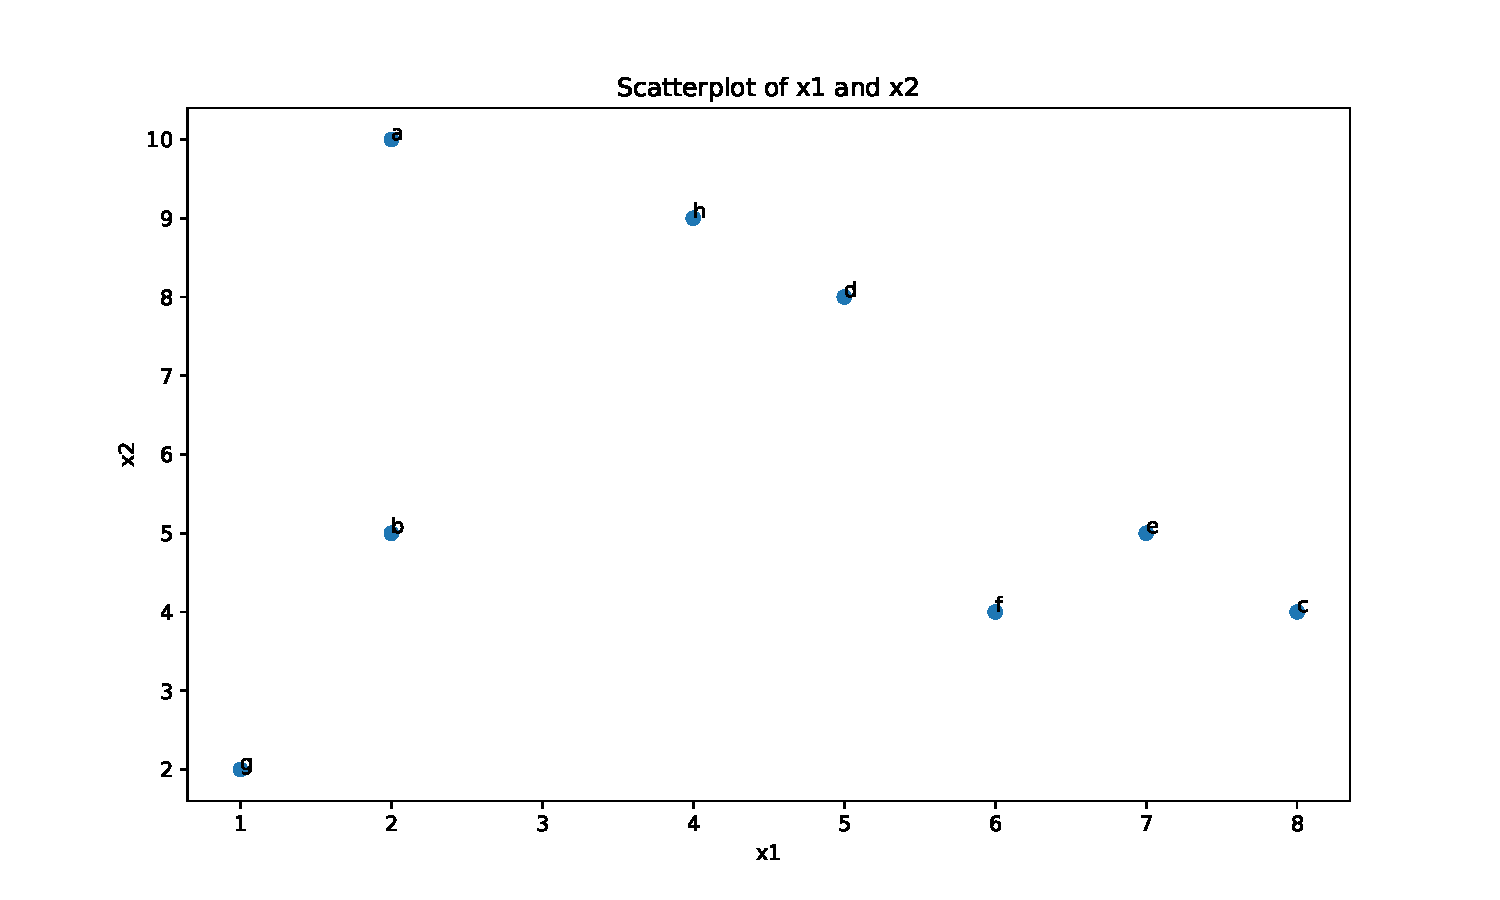
\includegraphics{dgetty_HW4_032224_files/figure-latex/Problem 3-1.pdf}
(a) If h and c are selected as the initial centers for your k-means
clustering, assign memberships for other points, and compute the means
(centroids) of your initial clusters. You can use Manhattan distance.

\begin{Shaded}
\begin{Highlighting}[]
\CommentTok{\# initial centers}
\NormalTok{c1 }\OperatorTok{=}\NormalTok{ P3\_df.loc[}\StringTok{\textquotesingle{}h\textquotesingle{}}\NormalTok{]}
\NormalTok{c2 }\OperatorTok{=}\NormalTok{ P3\_df.loc[}\StringTok{\textquotesingle{}c\textquotesingle{}}\NormalTok{]}
\BuiltInTok{print}\NormalTok{(c1)}
\end{Highlighting}
\end{Shaded}

x1 4 x2 9 Name: h, dtype: int64

\begin{Shaded}
\begin{Highlighting}[]
\BuiltInTok{print}\NormalTok{(c2)}
\end{Highlighting}
\end{Shaded}

x1 8 x2 4 Name: c, dtype: int64

\begin{Shaded}
\begin{Highlighting}[]
\CommentTok{\# assign memberships using manhattan distance}

\NormalTok{P3\_df[}\StringTok{\textquotesingle{}d\_c1\textquotesingle{}}\NormalTok{] }\OperatorTok{=}\NormalTok{ np.}\BuiltInTok{abs}\NormalTok{(P3\_df[}\StringTok{\textquotesingle{}x1\textquotesingle{}}\NormalTok{] }\OperatorTok{{-}}\NormalTok{ c1[}\StringTok{\textquotesingle{}x1\textquotesingle{}}\NormalTok{]) }\OperatorTok{+}\NormalTok{ np.}\BuiltInTok{abs}\NormalTok{(P3\_df[}\StringTok{\textquotesingle{}x2\textquotesingle{}}\NormalTok{] }\OperatorTok{{-}}\NormalTok{ c1[}\StringTok{\textquotesingle{}x2\textquotesingle{}}\NormalTok{])}
\NormalTok{P3\_df[}\StringTok{\textquotesingle{}d\_c2\textquotesingle{}}\NormalTok{] }\OperatorTok{=}\NormalTok{ np.}\BuiltInTok{abs}\NormalTok{(P3\_df[}\StringTok{\textquotesingle{}x1\textquotesingle{}}\NormalTok{] }\OperatorTok{{-}}\NormalTok{ c2[}\StringTok{\textquotesingle{}x1\textquotesingle{}}\NormalTok{]) }\OperatorTok{+}\NormalTok{ np.}\BuiltInTok{abs}\NormalTok{(P3\_df[}\StringTok{\textquotesingle{}x2\textquotesingle{}}\NormalTok{] }\OperatorTok{{-}}\NormalTok{ c2[}\StringTok{\textquotesingle{}x2\textquotesingle{}}\NormalTok{])}
\NormalTok{P3\_df[}\StringTok{\textquotesingle{}mem\textquotesingle{}}\NormalTok{] }\OperatorTok{=}\NormalTok{ np.where(P3\_df[}\StringTok{\textquotesingle{}d\_c1\textquotesingle{}}\NormalTok{] }\OperatorTok{\textless{}}\NormalTok{ P3\_df[}\StringTok{\textquotesingle{}d\_c2\textquotesingle{}}\NormalTok{], }\StringTok{\textquotesingle{}c1\textquotesingle{}}\NormalTok{, }\StringTok{\textquotesingle{}c2\textquotesingle{}}\NormalTok{)}

\CommentTok{\# P3\_df[\textquotesingle{}d\_c1\textquotesingle{}] = np.sqrt((P3\_df[\textquotesingle{}x1\textquotesingle{}] {-} c1[\textquotesingle{}x1\textquotesingle{}])**2 + (P3\_df[\textquotesingle{}x2\textquotesingle{}] {-} c1[\textquotesingle{}x2\textquotesingle{}])**2)}
\CommentTok{\# P3\_df[\textquotesingle{}d\_c2\textquotesingle{}] = np.sqrt((P3\_df[\textquotesingle{}x1\textquotesingle{}] {-} c2[\textquotesingle{}x1\textquotesingle{}])**2 + (P3\_df[\textquotesingle{}x2\textquotesingle{}] {-} c2[\textquotesingle{}x2\textquotesingle{}])**2)}
\CommentTok{\# P3\_df[\textquotesingle{}mem\textquotesingle{}] = np.where(P3\_df[\textquotesingle{}d\_c1\textquotesingle{}] \textless{} P3\_df[\textquotesingle{}d\_c2\textquotesingle{}], \textquotesingle{}c1\textquotesingle{}, \textquotesingle{}c2\textquotesingle{})}

\CommentTok{\# print(P3\_df)}
\BuiltInTok{print}\NormalTok{(P3\_df.to\_markdown(tablefmt}\OperatorTok{=}\StringTok{"grid"}\NormalTok{))}
\end{Highlighting}
\end{Shaded}

\begin{longtable}[]{@{}
  >{\raggedright\arraybackslash}p{(\columnwidth - 10\tabcolsep) * \real{0.0694}}
  >{\raggedright\arraybackslash}p{(\columnwidth - 10\tabcolsep) * \real{0.0972}}
  >{\raggedright\arraybackslash}p{(\columnwidth - 10\tabcolsep) * \real{0.0972}}
  >{\raggedright\arraybackslash}p{(\columnwidth - 10\tabcolsep) * \real{0.1250}}
  >{\raggedright\arraybackslash}p{(\columnwidth - 10\tabcolsep) * \real{0.1250}}
  >{\raggedright\arraybackslash}p{(\columnwidth - 10\tabcolsep) * \real{0.1111}}@{}}
\toprule\noalign{}
\begin{minipage}[b]{\linewidth}\raggedright
\end{minipage} & \begin{minipage}[b]{\linewidth}\raggedright
x1
\end{minipage} & \begin{minipage}[b]{\linewidth}\raggedright
x2
\end{minipage} & \begin{minipage}[b]{\linewidth}\raggedright
d\_c1
\end{minipage} & \begin{minipage}[b]{\linewidth}\raggedright
d\_c2
\end{minipage} & \begin{minipage}[b]{\linewidth}\raggedright
mem
\end{minipage} \\
\midrule\noalign{}
\endhead
\bottomrule\noalign{}
\endlastfoot
a & 2 & 10 & \begin{minipage}[t]{\linewidth}\raggedright
\begin{verbatim}
 3
\end{verbatim}
\end{minipage} & \begin{minipage}[t]{\linewidth}\raggedright
\begin{verbatim}
12
\end{verbatim}
\end{minipage} & c1 \\
b & 2 & 5 & \begin{minipage}[t]{\linewidth}\raggedright
\begin{verbatim}
 6
\end{verbatim}
\end{minipage} & \begin{minipage}[t]{\linewidth}\raggedright
\begin{verbatim}
 7
\end{verbatim}
\end{minipage} & c1 \\
c & 8 & 4 & \begin{minipage}[t]{\linewidth}\raggedright
\begin{verbatim}
 9
\end{verbatim}
\end{minipage} & \begin{minipage}[t]{\linewidth}\raggedright
\begin{verbatim}
 0
\end{verbatim}
\end{minipage} & c2 \\
d & 5 & 8 & \begin{minipage}[t]{\linewidth}\raggedright
\begin{verbatim}
 2
\end{verbatim}
\end{minipage} & \begin{minipage}[t]{\linewidth}\raggedright
\begin{verbatim}
 7
\end{verbatim}
\end{minipage} & c1 \\
e & 7 & 5 & \begin{minipage}[t]{\linewidth}\raggedright
\begin{verbatim}
 7
\end{verbatim}
\end{minipage} & \begin{minipage}[t]{\linewidth}\raggedright
\begin{verbatim}
 2
\end{verbatim}
\end{minipage} & c2 \\
f & 6 & 4 & \begin{minipage}[t]{\linewidth}\raggedright
\begin{verbatim}
 7
\end{verbatim}
\end{minipage} & \begin{minipage}[t]{\linewidth}\raggedright
\begin{verbatim}
 2
\end{verbatim}
\end{minipage} & c2 \\
g & 1 & 2 & \begin{minipage}[t]{\linewidth}\raggedright
\begin{verbatim}
10
\end{verbatim}
\end{minipage} & \begin{minipage}[t]{\linewidth}\raggedright
\begin{verbatim}
 9
\end{verbatim}
\end{minipage} & c2 \\
h & 4 & 9 & \begin{minipage}[t]{\linewidth}\raggedright
\begin{verbatim}
 0
\end{verbatim}
\end{minipage} & \begin{minipage}[t]{\linewidth}\raggedright
\begin{verbatim}
 9
\end{verbatim}
\end{minipage} & c1 \\
\end{longtable}

\begin{Shaded}
\begin{Highlighting}[]
\CommentTok{\# build a visualization of the k{-}means clustering}
\NormalTok{plt.figure(figsize}\OperatorTok{=}\NormalTok{(}\DecValTok{10}\NormalTok{, }\DecValTok{6}\NormalTok{))}
\NormalTok{plt.scatter(P3\_df[}\StringTok{\textquotesingle{}x1\textquotesingle{}}\NormalTok{], P3\_df[}\StringTok{\textquotesingle{}x2\textquotesingle{}}\NormalTok{], c}\OperatorTok{=}\NormalTok{P3\_df[}\StringTok{\textquotesingle{}mem\textquotesingle{}}\NormalTok{].}\BuiltInTok{map}\NormalTok{(\{}\StringTok{\textquotesingle{}c1\textquotesingle{}}\NormalTok{: }\StringTok{\textquotesingle{}red\textquotesingle{}}\NormalTok{, }\StringTok{\textquotesingle{}c2\textquotesingle{}}\NormalTok{: }\StringTok{\textquotesingle{}blue\textquotesingle{}}\NormalTok{\}))}
\NormalTok{plt.scatter(c1[}\StringTok{\textquotesingle{}x1\textquotesingle{}}\NormalTok{], c1[}\StringTok{\textquotesingle{}x2\textquotesingle{}}\NormalTok{], color}\OperatorTok{=}\StringTok{\textquotesingle{}red\textquotesingle{}}\NormalTok{, marker}\OperatorTok{=}\StringTok{\textquotesingle{}x\textquotesingle{}}\NormalTok{, s}\OperatorTok{=}\DecValTok{100}\NormalTok{)}
\NormalTok{plt.scatter(c2[}\StringTok{\textquotesingle{}x1\textquotesingle{}}\NormalTok{], c2[}\StringTok{\textquotesingle{}x2\textquotesingle{}}\NormalTok{], color}\OperatorTok{=}\StringTok{\textquotesingle{}blue\textquotesingle{}}\NormalTok{, marker}\OperatorTok{=}\StringTok{\textquotesingle{}x\textquotesingle{}}\NormalTok{, s}\OperatorTok{=}\DecValTok{100}\NormalTok{)}
\NormalTok{plt.xlabel(}\StringTok{\textquotesingle{}x1\textquotesingle{}}\NormalTok{)}
\NormalTok{plt.ylabel(}\StringTok{\textquotesingle{}x2\textquotesingle{}}\NormalTok{)}
\NormalTok{plt.title(}\StringTok{\textquotesingle{}Scatterplot of x1 and x2 with k{-}means clustering\textquotesingle{}}\NormalTok{)}
\ControlFlowTok{for}\NormalTok{ i, txt }\KeywordTok{in} \BuiltInTok{enumerate}\NormalTok{(classes):}
\NormalTok{    plt.annotate(txt, (P3\_df[}\StringTok{\textquotesingle{}x1\textquotesingle{}}\NormalTok{][i], P3\_df[}\StringTok{\textquotesingle{}x2\textquotesingle{}}\NormalTok{][i]))}

\NormalTok{plt.show()}
\end{Highlighting}
\end{Shaded}

\includegraphics{dgetty_HW4_032224_files/figure-latex/Problem 3a-3.pdf}

\begin{enumerate}
\def\labelenumi{(\alph{enumi})}
\setcounter{enumi}{1}
\tightlist
\item
  Based on the centroids you found above reassign the memberships by
  using Manhattan distance
\end{enumerate}

\begin{Shaded}
\begin{Highlighting}[]
\CommentTok{\# reassign memberships}
\NormalTok{c1 }\OperatorTok{=}\NormalTok{ P3\_df[P3\_df[}\StringTok{\textquotesingle{}mem\textquotesingle{}}\NormalTok{] }\OperatorTok{==} \StringTok{\textquotesingle{}c1\textquotesingle{}}\NormalTok{][[}\StringTok{\textquotesingle{}x1\textquotesingle{}}\NormalTok{, }\StringTok{\textquotesingle{}x2\textquotesingle{}}\NormalTok{]].mean()}
\NormalTok{c2 }\OperatorTok{=}\NormalTok{ P3\_df[P3\_df[}\StringTok{\textquotesingle{}mem\textquotesingle{}}\NormalTok{] }\OperatorTok{==} \StringTok{\textquotesingle{}c2\textquotesingle{}}\NormalTok{][[}\StringTok{\textquotesingle{}x1\textquotesingle{}}\NormalTok{, }\StringTok{\textquotesingle{}x2\textquotesingle{}}\NormalTok{]].mean()}

\NormalTok{P3\_df[}\StringTok{\textquotesingle{}d\_c1\textquotesingle{}}\NormalTok{] }\OperatorTok{=}\NormalTok{ np.}\BuiltInTok{abs}\NormalTok{(P3\_df[}\StringTok{\textquotesingle{}x1\textquotesingle{}}\NormalTok{] }\OperatorTok{{-}}\NormalTok{ c1[}\StringTok{\textquotesingle{}x1\textquotesingle{}}\NormalTok{]) }\OperatorTok{+}\NormalTok{ np.}\BuiltInTok{abs}\NormalTok{(P3\_df[}\StringTok{\textquotesingle{}x2\textquotesingle{}}\NormalTok{] }\OperatorTok{{-}}\NormalTok{ c1[}\StringTok{\textquotesingle{}x2\textquotesingle{}}\NormalTok{])}
\NormalTok{P3\_df[}\StringTok{\textquotesingle{}d\_c2\textquotesingle{}}\NormalTok{] }\OperatorTok{=}\NormalTok{ np.}\BuiltInTok{abs}\NormalTok{(P3\_df[}\StringTok{\textquotesingle{}x1\textquotesingle{}}\NormalTok{] }\OperatorTok{{-}}\NormalTok{ c2[}\StringTok{\textquotesingle{}x1\textquotesingle{}}\NormalTok{]) }\OperatorTok{+}\NormalTok{ np.}\BuiltInTok{abs}\NormalTok{(P3\_df[}\StringTok{\textquotesingle{}x2\textquotesingle{}}\NormalTok{] }\OperatorTok{{-}}\NormalTok{ c2[}\StringTok{\textquotesingle{}x2\textquotesingle{}}\NormalTok{])}
\NormalTok{P3\_df[}\StringTok{\textquotesingle{}mem\textquotesingle{}}\NormalTok{] }\OperatorTok{=}\NormalTok{ np.where(P3\_df[}\StringTok{\textquotesingle{}d\_c1\textquotesingle{}}\NormalTok{] }\OperatorTok{\textless{}}\NormalTok{ P3\_df[}\StringTok{\textquotesingle{}d\_c2\textquotesingle{}}\NormalTok{], }\StringTok{\textquotesingle{}c1\textquotesingle{}}\NormalTok{, }\StringTok{\textquotesingle{}c2\textquotesingle{}}\NormalTok{)}

\CommentTok{\# P3\_df[\textquotesingle{}d\_c1\textquotesingle{}] = np.sqrt((P3\_df[\textquotesingle{}x1\textquotesingle{}] {-} c1[\textquotesingle{}x1\textquotesingle{}])**2 + (P3\_df[\textquotesingle{}x2\textquotesingle{}] {-} c1[\textquotesingle{}x2\textquotesingle{}])**2)}
\CommentTok{\# P3\_df[\textquotesingle{}d\_c2\textquotesingle{}] = np.sqrt((P3\_df[\textquotesingle{}x1\textquotesingle{}] {-} c2[\textquotesingle{}x1\textquotesingle{}])**2 + (P3\_df[\textquotesingle{}x2\textquotesingle{}] {-} c2[\textquotesingle{}x2\textquotesingle{}])**2)}
\CommentTok{\# P3\_df[\textquotesingle{}mem\textquotesingle{}] = np.where(P3\_df[\textquotesingle{}d\_c1\textquotesingle{}] \textless{} P3\_df[\textquotesingle{}d\_c2\textquotesingle{}], \textquotesingle{}c1\textquotesingle{}, \textquotesingle{}c2\textquotesingle{})}

\CommentTok{\# print(P3\_df)}
\BuiltInTok{print}\NormalTok{(P3\_df.to\_markdown(tablefmt}\OperatorTok{=}\StringTok{"grid"}\NormalTok{))}
\end{Highlighting}
\end{Shaded}

\begin{longtable}[]{@{}
  >{\raggedright\arraybackslash}p{(\columnwidth - 10\tabcolsep) * \real{0.0694}}
  >{\raggedright\arraybackslash}p{(\columnwidth - 10\tabcolsep) * \real{0.0972}}
  >{\raggedright\arraybackslash}p{(\columnwidth - 10\tabcolsep) * \real{0.0972}}
  >{\raggedright\arraybackslash}p{(\columnwidth - 10\tabcolsep) * \real{0.1250}}
  >{\raggedright\arraybackslash}p{(\columnwidth - 10\tabcolsep) * \real{0.1250}}
  >{\raggedright\arraybackslash}p{(\columnwidth - 10\tabcolsep) * \real{0.1111}}@{}}
\toprule\noalign{}
\begin{minipage}[b]{\linewidth}\raggedright
\end{minipage} & \begin{minipage}[b]{\linewidth}\raggedright
x1
\end{minipage} & \begin{minipage}[b]{\linewidth}\raggedright
x2
\end{minipage} & \begin{minipage}[b]{\linewidth}\raggedright
d\_c1
\end{minipage} & \begin{minipage}[b]{\linewidth}\raggedright
d\_c2
\end{minipage} & \begin{minipage}[b]{\linewidth}\raggedright
mem
\end{minipage} \\
\midrule\noalign{}
\endhead
\bottomrule\noalign{}
\endlastfoot
a & 2 & 10 & 3.25 & 9.75 & c1 \\
b & 2 & 5 & 4.25 & 4.75 & c1 \\
c & 8 & 4 & 8.75 & 2.75 & c2 \\
d & 5 & 8 & 1.75 & 4.75 & c1 \\
e & 7 & 5 & 6.75 & 2.75 & c2 \\
f & 6 & 4 & 6.75 & 0.75 & c2 \\
g & 1 & 2 & 8.25 & 6.25 & c2 \\
h & 4 & 9 & 1.75 & 6.75 & c1 \\
\end{longtable}

\begin{Shaded}
\begin{Highlighting}[]
\CommentTok{\# build a visualization of the reassigned k{-}means clustering}
\NormalTok{plt.figure(figsize}\OperatorTok{=}\NormalTok{(}\DecValTok{10}\NormalTok{, }\DecValTok{6}\NormalTok{))}
\NormalTok{plt.scatter(P3\_df[}\StringTok{\textquotesingle{}x1\textquotesingle{}}\NormalTok{], P3\_df[}\StringTok{\textquotesingle{}x2\textquotesingle{}}\NormalTok{], c}\OperatorTok{=}\NormalTok{P3\_df[}\StringTok{\textquotesingle{}mem\textquotesingle{}}\NormalTok{].}\BuiltInTok{map}\NormalTok{(\{}\StringTok{\textquotesingle{}c1\textquotesingle{}}\NormalTok{: }\StringTok{\textquotesingle{}red\textquotesingle{}}\NormalTok{, }\StringTok{\textquotesingle{}c2\textquotesingle{}}\NormalTok{: }\StringTok{\textquotesingle{}blue\textquotesingle{}}\NormalTok{\}))}
\NormalTok{plt.scatter(c1[}\StringTok{\textquotesingle{}x1\textquotesingle{}}\NormalTok{], c1[}\StringTok{\textquotesingle{}x2\textquotesingle{}}\NormalTok{], color}\OperatorTok{=}\StringTok{\textquotesingle{}red\textquotesingle{}}\NormalTok{, marker}\OperatorTok{=}\StringTok{\textquotesingle{}x\textquotesingle{}}\NormalTok{, s}\OperatorTok{=}\DecValTok{100}\NormalTok{)}
\NormalTok{plt.scatter(c2[}\StringTok{\textquotesingle{}x1\textquotesingle{}}\NormalTok{], c2[}\StringTok{\textquotesingle{}x2\textquotesingle{}}\NormalTok{], color}\OperatorTok{=}\StringTok{\textquotesingle{}blue\textquotesingle{}}\NormalTok{, marker}\OperatorTok{=}\StringTok{\textquotesingle{}x\textquotesingle{}}\NormalTok{, s}\OperatorTok{=}\DecValTok{100}\NormalTok{)}
\NormalTok{plt.xlabel(}\StringTok{\textquotesingle{}x1\textquotesingle{}}\NormalTok{)}
\NormalTok{plt.ylabel(}\StringTok{\textquotesingle{}x2\textquotesingle{}}\NormalTok{)}
\NormalTok{plt.title(}\StringTok{\textquotesingle{}Scatterplot of x1 and x2 with reassigned k{-}means clustering\textquotesingle{}}\NormalTok{)}
\ControlFlowTok{for}\NormalTok{ i, txt }\KeywordTok{in} \BuiltInTok{enumerate}\NormalTok{(classes):}
\NormalTok{    plt.annotate(txt, (P3\_df[}\StringTok{\textquotesingle{}x1\textquotesingle{}}\NormalTok{][i], P3\_df[}\StringTok{\textquotesingle{}x2\textquotesingle{}}\NormalTok{][i]))}
    
\NormalTok{plt.show()}
\end{Highlighting}
\end{Shaded}

\includegraphics{dgetty_HW4_032224_files/figure-latex/Problem 3b-5.pdf}

\begin{enumerate}
\def\labelenumi{\arabic{enumi}.}
\setcounter{enumi}{3}
\tightlist
\item
  Given the distance matrix below answer the following questions. Notice
  that this is a distance matrix, meaning the distance between any pair
  of points can be found by checking the corresponding cell.
\end{enumerate}

\begin{Shaded}
\begin{Highlighting}[]
\CommentTok{\# create a data frame}
\NormalTok{classes }\OperatorTok{=}\NormalTok{ [}\StringTok{\textquotesingle{}b\textquotesingle{}}\NormalTok{,}\StringTok{\textquotesingle{}c\textquotesingle{}}\NormalTok{,}\StringTok{\textquotesingle{}d\textquotesingle{}}\NormalTok{,}\StringTok{\textquotesingle{}e\textquotesingle{}}\NormalTok{,}\StringTok{\textquotesingle{}f\textquotesingle{}}\NormalTok{,}\StringTok{\textquotesingle{}g\textquotesingle{}}\NormalTok{,}\StringTok{\textquotesingle{}h\textquotesingle{}}\NormalTok{]}
\NormalTok{data }\OperatorTok{=}\NormalTok{ \{}\StringTok{\textquotesingle{}a\textquotesingle{}}\NormalTok{: [}\DecValTok{5}\NormalTok{, }\DecValTok{8}\NormalTok{, }\DecValTok{4}\NormalTok{, }\DecValTok{7}\NormalTok{, }\DecValTok{7}\NormalTok{, }\DecValTok{8}\NormalTok{, }\DecValTok{2}\NormalTok{],}\StringTok{\textquotesingle{}b\textquotesingle{}}\NormalTok{: [}\DecValTok{0}\NormalTok{, }\DecValTok{6}\NormalTok{, }\DecValTok{4}\NormalTok{, }\DecValTok{5}\NormalTok{, }\DecValTok{4}\NormalTok{, }\DecValTok{3}\NormalTok{, }\DecValTok{4}\NormalTok{],}\StringTok{\textquotesingle{}c\textquotesingle{}}\NormalTok{: [}\DecValTok{0}\NormalTok{, }\DecValTok{0}\NormalTok{, }\DecValTok{5}\NormalTok{, }\DecValTok{1}\NormalTok{, }\DecValTok{2}\NormalTok{, }\DecValTok{7}\NormalTok{, }\DecValTok{6}\NormalTok{],}\StringTok{\textquotesingle{}d\textquotesingle{}}\NormalTok{: [}\DecValTok{0}\NormalTok{, }\DecValTok{0}\NormalTok{, }\DecValTok{0}\NormalTok{, }\DecValTok{4}\NormalTok{, }\DecValTok{4}\NormalTok{, }\DecValTok{7}\NormalTok{, }\DecValTok{1}\NormalTok{],}\StringTok{\textquotesingle{}e\textquotesingle{}}\NormalTok{: [}\DecValTok{0}\NormalTok{,}\DecValTok{0}\NormalTok{, }\DecValTok{0}\NormalTok{, }\DecValTok{0}\NormalTok{, }\DecValTok{1}\NormalTok{, }\DecValTok{7}\NormalTok{, }\DecValTok{5}\NormalTok{],}\StringTok{\textquotesingle{}f\textquotesingle{}}\NormalTok{: [}\DecValTok{0}\NormalTok{, }\DecValTok{0}\NormalTok{, }\DecValTok{0}\NormalTok{, }\DecValTok{0}\NormalTok{, }\DecValTok{0}\NormalTok{, }\DecValTok{5}\NormalTok{, }\DecValTok{5}\NormalTok{],}\StringTok{\textquotesingle{}g\textquotesingle{}}\NormalTok{: [}\DecValTok{0}\NormalTok{, }\DecValTok{0}\NormalTok{, }\DecValTok{0}\NormalTok{, }\DecValTok{0}\NormalTok{, }\DecValTok{0}\NormalTok{, }\DecValTok{0}\NormalTok{, }\DecValTok{8}\NormalTok{]\}}
\NormalTok{P4\_df }\OperatorTok{=}\NormalTok{ pd.DataFrame(data, index}\OperatorTok{=}\NormalTok{classes)}
\CommentTok{\# print(P4\_df)}
\BuiltInTok{print}\NormalTok{(P4\_df.to\_markdown(tablefmt}\OperatorTok{=}\StringTok{"grid"}\NormalTok{))}
\end{Highlighting}
\end{Shaded}

\begin{longtable}[]{@{}
  >{\raggedright\arraybackslash}p{(\columnwidth - 14\tabcolsep) * \real{0.0694}}
  >{\raggedright\arraybackslash}p{(\columnwidth - 14\tabcolsep) * \real{0.0833}}
  >{\raggedright\arraybackslash}p{(\columnwidth - 14\tabcolsep) * \real{0.0833}}
  >{\raggedright\arraybackslash}p{(\columnwidth - 14\tabcolsep) * \real{0.0833}}
  >{\raggedright\arraybackslash}p{(\columnwidth - 14\tabcolsep) * \real{0.0833}}
  >{\raggedright\arraybackslash}p{(\columnwidth - 14\tabcolsep) * \real{0.0833}}
  >{\raggedright\arraybackslash}p{(\columnwidth - 14\tabcolsep) * \real{0.0833}}
  >{\raggedright\arraybackslash}p{(\columnwidth - 14\tabcolsep) * \real{0.0833}}@{}}
\toprule\noalign{}
\begin{minipage}[b]{\linewidth}\raggedright
\end{minipage} & \begin{minipage}[b]{\linewidth}\raggedright
a
\end{minipage} & \begin{minipage}[b]{\linewidth}\raggedright
b
\end{minipage} & \begin{minipage}[b]{\linewidth}\raggedright
c
\end{minipage} & \begin{minipage}[b]{\linewidth}\raggedright
d
\end{minipage} & \begin{minipage}[b]{\linewidth}\raggedright
e
\end{minipage} & \begin{minipage}[b]{\linewidth}\raggedright
f
\end{minipage} & \begin{minipage}[b]{\linewidth}\raggedright
g
\end{minipage} \\
\midrule\noalign{}
\endhead
\bottomrule\noalign{}
\endlastfoot
b & 5 & 0 & 0 & 0 & 0 & 0 & 0 \\
c & 8 & 6 & 0 & 0 & 0 & 0 & 0 \\
d & 4 & 4 & 5 & 0 & 0 & 0 & 0 \\
e & 7 & 5 & 1 & 4 & 0 & 0 & 0 \\
f & 7 & 4 & 2 & 4 & 1 & 0 & 0 \\
g & 8 & 3 & 7 & 7 & 7 & 5 & 0 \\
h & 2 & 4 & 6 & 1 & 5 & 5 & 8 \\
\end{longtable}

\begin{enumerate}
\def\labelenumi{(\alph{enumi})}
\tightlist
\item
  Apply the hierarchical clustering algorithm with single linkage to the
  data above. Draw the final dendrogram.
\end{enumerate}

\begin{Shaded}
\begin{Highlighting}[]
\CommentTok{\# apply hierarchical clustering with single linkage}
\ImportTok{from}\NormalTok{ scipy.cluster.hierarchy }\ImportTok{import}\NormalTok{ linkage, dendrogram}
\NormalTok{Z }\OperatorTok{=}\NormalTok{ linkage(P4\_df, }\StringTok{\textquotesingle{}single\textquotesingle{}}\NormalTok{)}
\NormalTok{plt.figure(figsize}\OperatorTok{=}\NormalTok{(}\DecValTok{10}\NormalTok{, }\DecValTok{6}\NormalTok{))}
\NormalTok{dendrogram(Z, p}\OperatorTok{=}\DecValTok{30}\NormalTok{, truncate\_mode}\OperatorTok{=}\VariableTok{None}\NormalTok{, color\_threshold}\OperatorTok{=}\VariableTok{None}\NormalTok{, get\_leaves}\OperatorTok{=}\VariableTok{True}\NormalTok{, orientation}\OperatorTok{=}\StringTok{\textquotesingle{}top\textquotesingle{}}\NormalTok{, labels}\OperatorTok{=}\NormalTok{classes, count\_sort}\OperatorTok{=}\VariableTok{False}\NormalTok{, distance\_sort}\OperatorTok{=}\VariableTok{False}\NormalTok{, show\_leaf\_counts}\OperatorTok{=}\VariableTok{True}\NormalTok{, no\_plot}\OperatorTok{=}\VariableTok{False}\NormalTok{, no\_labels}\OperatorTok{=}\VariableTok{False}\NormalTok{, leaf\_font\_size}\OperatorTok{=}\VariableTok{None}\NormalTok{, leaf\_rotation}\OperatorTok{=}\VariableTok{None}\NormalTok{, leaf\_label\_func}\OperatorTok{=}\VariableTok{None}\NormalTok{, show\_contracted}\OperatorTok{=}\VariableTok{False}\NormalTok{, link\_color\_func}\OperatorTok{=}\VariableTok{None}\NormalTok{, ax}\OperatorTok{=}\VariableTok{None}\NormalTok{, above\_threshold\_color}\OperatorTok{=}\StringTok{\textquotesingle{}C0\textquotesingle{}}\NormalTok{)}
\end{Highlighting}
\end{Shaded}

\{`icoord': {[}{[}55.0, 55.0, 65.0, 65.0{]}, {[}45.0, 45.0, 60.0,
60.0{]}, {[}35.0, 35.0, 52.5, 52.5{]}, {[}25.0, 25.0, 43.75, 43.75{]},
{[}15.0, 15.0, 34.375, 34.375{]}, {[}5.0, 5.0, 24.6875, 24.6875{]}{]},
`dcoord': {[}{[}0.0, 1.7320508075688772, 1.7320508075688772, 0.0{]},
{[}0.0, 4.358898943540674, 4.358898943540674, 1.7320508075688772{]},
{[}0.0, 5.916079783099616, 5.916079783099616, 4.358898943540674{]},
{[}0.0, 6.4031242374328485, 6.4031242374328485, 5.916079783099616{]},
{[}0.0, 9.848857801796104, 9.848857801796104, 6.4031242374328485{]},
{[}0.0, 10.954451150103322, 10.954451150103322, 9.848857801796104{]}{]},
`ivl': {[}`h', `g', `b', `d', `c', `e', `f'{]}, `leaves': {[}6, 5, 0, 2,
1, 3, 4{]}, `color\_list': {[}`C1', `C1', `C1', `C1', `C0', `C0'{]},
`leaves\_color\_list': {[}`C0', `C0', `C1', `C1', `C1', `C1', `C1'{]}\}

\begin{Shaded}
\begin{Highlighting}[]
\NormalTok{plt.title(}\StringTok{\textquotesingle{}Dendrogram of hierarchical clustering with single linkage\textquotesingle{}}\NormalTok{)}
\NormalTok{plt.show()}
\end{Highlighting}
\end{Shaded}

\includegraphics{dgetty_HW4_032224_files/figure-latex/Problem 4a-7.pdf}

\begin{enumerate}
\def\labelenumi{(\alph{enumi})}
\setcounter{enumi}{1}
\tightlist
\item
  Determine whether a point is core based on eps = 6 and `minPts' = 2.
  (Recall that a point p is a core point if at least `minPts' points are
  within distance eps of it (including p).
\end{enumerate}

\begin{Shaded}
\begin{Highlighting}[]
\CommentTok{\# determine core points}
\NormalTok{eps }\OperatorTok{=} \DecValTok{6}
\NormalTok{minPts }\OperatorTok{=} \DecValTok{2}
\NormalTok{core\_points }\OperatorTok{=}\NormalTok{ []}
\ControlFlowTok{for}\NormalTok{ i }\KeywordTok{in} \BuiltInTok{range}\NormalTok{(}\BuiltInTok{len}\NormalTok{(P4\_df)):}
    \ControlFlowTok{if} \BuiltInTok{sum}\NormalTok{(P4\_df.iloc[i] }\OperatorTok{\textless{}=}\NormalTok{ eps) }\OperatorTok{\textgreater{}=}\NormalTok{ minPts:}
\NormalTok{        core\_points.append(classes[i])}
        
\BuiltInTok{print}\NormalTok{(}\StringTok{"Core Points:"}\NormalTok{,core\_points)}
\end{Highlighting}
\end{Shaded}

Core Points: {[}`b', `c', `d', `e', `f', `g', `h'{]}

\end{document}
